%%%%%%%%%%%%%%%%%%%%%%%%%%%%%%%%%%%%%%%%%%%%%%%%%%%%%%%%%%%%%%%%%%%%%%%%%%%%%%%
% Schematische Darstellung eines Rolling Horizon
%%%%%%%%%%%%%%%%%%%%%%%%%%%%%%%%%%%%%%%%%%%%%%%%%%%%%%%%%%%%%%%%%%%%%%%%%%%%%%%

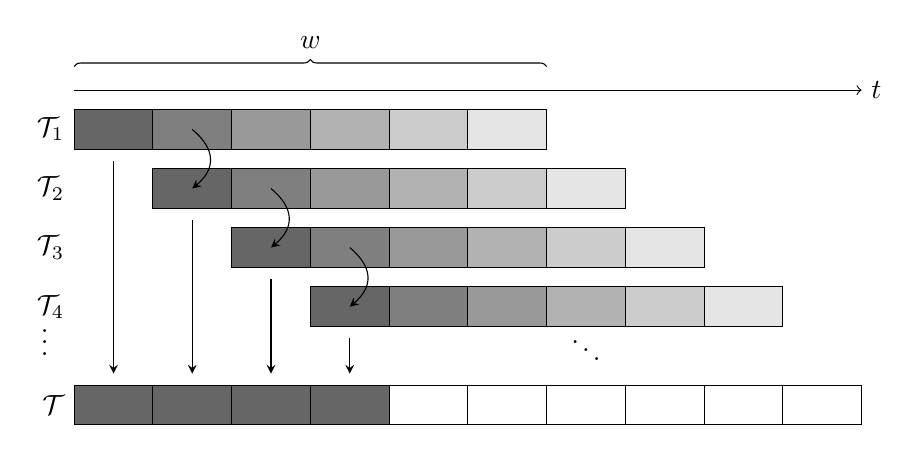
\begin{tikzpicture}
	\draw[->] (0,0) -- (10,0) node[right]{$t$};
	% 1. Horizont
	\node[left] at (0,-0.5) {$\mathcal{T}_1$};
	\foreach \x in {0,1,...,5}{
		\draw(\x,-.75) rectangle (\x+1,-.25);
		\fill[black, opacity={0.6-\x/10}](\x,-.75) rectangle (\x+1,-.25);
	}
	\draw[-stealth] (1.5,-0.5) .. controls (1.8,-.75) and (1.8,-1)
	.. (1.5,-1.25);
		
	% 2. Horizont
	\node[left] at (0,-1.25) {$\mathcal{T}_2$};
	\foreach \x in {1,2,...,6}{
		\draw(\x,-1.5) rectangle (\x+1,-1);
		\fill[black, opacity={0.7-\x/10}](\x,-1.5) rectangle (\x+1,-1);
	}
	\draw[-stealth] (2.5,-1.25) .. controls (2.8,-1.5) and (2.8,-1.75) 
	.. (2.5,-2);
		
	% 3. Horizont
	\node[left] at (0,-2) {$\mathcal{T}_3$};
	\foreach \x in {2,3,...,7}{
		\draw (\x,-2.25) rectangle (\x+1,-1.75);
		\fill[black, opacity={0.8-\x/10}](\x,-2.25) rectangle (\x+1,-1.75);
	}
	\draw[-stealth] (3.5,-2) .. controls (3.8,-2.25) and (3.8,-2.5) 
	.. (3.5,-2.75);
	
	% 4. Horizont
	\node[left] at (0,-2.75) {$\mathcal{T}_4$};
	\foreach \x in {3,4,...,8}{
		\draw (\x,-3) rectangle (\x+1,-2.5);
		\fill[black, opacity={0.9-\x/10}](\x,-3) rectangle (\x+1,-2.5);
	}
	
	% oben geschweifte Klammer, welche die Weite eines Horizonts angibt
	\draw[decorate, decoration=brace] (0, 0.3) -- (6, 0.3)
	node[pos=0.5, above=1mm]{$w$};
		
	% unten das Ergebnis zeichnen
	\node[left] at (0,-4) {$\mathcal{T}$};
	\foreach \x in {0,1,...,9}{
		\draw (\x,-3.75) rectangle (\x+1,-4.25);
	}
	
	\foreach \x in {0,1,...,3}{
		\fill[black, opacity={0.6}] (\x,-3.75) rectangle (\x+1,-4.25);
	}
	
	% Pfeile, die anzeigen, dass die jeweils ersten Ergebnisse von
	% den Horizonten übernommen werden
	\draw[-stealth] (0.5,-0.9) -- (0.5,-3.6);
	\draw[-stealth] (1.5,-1.65) -- (1.5,-3.6);
	\draw[-stealth] (2.5,-2.4) -- (2.5,-3.6);
	\draw[-stealth] (3.5,-3.15) -- (3.5,-3.6);
	
	% diagonale Pünktchen, die andeuten, dass noch mehr Horizonte folgen
	\node at (6.5,-3.2){$\ddots$};
	\node[left] at (-0.2,-3.1){$\vdots$};
	
\end{tikzpicture}